\section{Unsupervised Learning and Mining}

\subsection{Introduction to Unsupervised Learning}

\begin{definition}{Unsupervised Learning}\\
In unsupervised learning, the training data does not contain any output (target) values. The goal is to model the underlying distribution of the data to describe its structure, discover hidden patterns, and gain insights.
\end{definition}

\subsection{Introduction to Clustering}

\begin{definition}{Clustering}\\
Clustering is the task of grouping a set of objects in such a way that objects in the same group (called a cluster) are more similar to each other than to objects in other groups. Given a set of $M$ data points $X = \{x^{(1)}, x^{(2)}, \ldots, x^{(M)}\}$, where each data point consists of $N$ features $x^{(i)} = (x^{(i)}_1, \ldots, x^{(i)}_N) \in \mathbb{R}^N$, and a distance measure $d$, a clustering algorithm separates the data into $K$ clusters.
\end{definition}

\begin{concept}{Types of Clustering}\\
There are two main types of clustering:
\begin{itemize}
    \item \textbf{Hard Clustering}: Each data point is assigned to exactly one cluster
    \item \textbf{Soft Clustering}: Each data point is assigned a probability or membership degree for each cluster
\end{itemize}
\end{concept}

\begin{example}{Clustering Application}
Customer segmentation for targeted marketing:
\begin{itemize}
    \item Data: Customer purchase history, demographics, website behavior
    \item Clustering reveals natural customer segments:
    \begin{itemize}
        \item Cluster 1: Young, high-income professionals who buy luxury items
        \item Cluster 2: Middle-aged parents who focus on household essentials
        \item Cluster 3: Budget-conscious shoppers who primarily buy discounted items
    \end{itemize}
    \item Marketing strategies can be tailored to each segment
\end{itemize}
\end{example}

\subsection{K-Means Algorithm}

\begin{definition}{K-Means Algorithm}\\
K-means is a clustering algorithm that aims to partition $M$ data points into $K$ clusters, where each data point belongs to the cluster with the nearest mean (centroid). The algorithm minimizes the within-cluster sum of squares (inertia):
\[\sum_{k=1}^{K} \sum_{x^{(i)} \in C_k} ||x^{(i)} - \mu_k||^2\]
where $C_k$ is the set of points in cluster $k$ and $\mu_k$ is the centroid of cluster $k$.

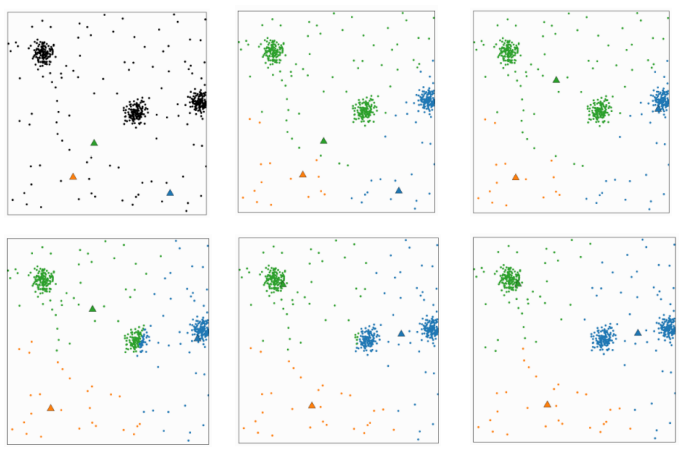
\includegraphics[width=0.7\linewidth]{kmeans_simpleKR.png}
\end{definition}


\begin{KR}{Implementing K-Means}
\paragraph{Initialize centroids}
Choose $K$ initial centroids:
\begin{itemize}
    \item Random selection: Randomly select $K$ data points
    \item K-means++: Select centroids that are farther apart
\end{itemize}

\paragraph{Assign points to closest centroid}
For each data point $x^{(i)}$:
\begin{itemize}
    \item Calculate distance to each centroid
    \item Assign the point to the closest centroid's cluster
\end{itemize}

\paragraph{Update centroids}
For each cluster $k$:
\begin{itemize}
    \item Calculate the mean of all points in the cluster
    \item Set the new centroid to this mean: $\mu_k = \frac{1}{|C_k|} \sum_{x^{(i)} \in C_k} x^{(i)}$
\end{itemize}

\paragraph{Repeat until convergence}
Repeat steps 2 and 3 until:
\begin{itemize}
    \item Centroids no longer change significantly
    \item Maximum number of iterations is reached
    \item Assignment of points to clusters stabilizes
\end{itemize}
\end{KR}

\begin{example2}{K-Means Step-by-Step}\\
Consider a dataset with six 2D points: (1,1), (2,1), (4,3), (5,4), (1,2), (2,2)
\begin{itemize}
    \item Initialize $K=2$ centroids: $\mu_1 = (1,1)$ and $\mu_2 = (5,4)$
\end{itemize}
\tcblower
Iteration 1:
\begin{itemize}
    \item Assign points to clusters:
    \begin{itemize}
        \item Cluster 1: (1,1), (2,1), (1,2), (2,2) [closer to $\mu_1$]
        \item Cluster 2: (4,3), (5,4) [closer to $\mu_2$]
    \end{itemize}
    \item Update centroids:
    \begin{itemize}
        \item $\mu_1 = \frac{(1,1) + (2,1) + (1,2) + (2,2)}{4} = (1.5, 1.5)$
        \item $\mu_2 = \frac{(4,3) + (5,4)}{2} = (4.5, 3.5)$
    \end{itemize}
\end{itemize}

Iteration 2:
\begin{itemize}
    \item Assign points to clusters:
    \begin{itemize}
        \item Cluster 1: (1,1), (2,1), (1,2), (2,2) [closer to $\mu_1$]
        \item Cluster 2: (4,3), (5,4) [closer to $\mu_2$]
    \end{itemize}
    \item The assignments haven't changed, so the algorithm has converged
\end{itemize}

Final clusters:
\begin{itemize}
    \item Cluster 1: (1,1), (2,1), (1,2), (2,2) with centroid (1.5, 1.5)
    \item Cluster 2: (4,3), (5,4) with centroid (4.5, 3.5)
\end{itemize}
\end{example2}

\begin{definition}{K-means++}\\
K-means++ is an initialization method for K-means that selects initial centroids that are far away from each other:
\begin{enumerate}
    \item Choose the first centroid randomly from the data points
    \item For each subsequent centroid, select a data point with probability proportional to the squared distance to the nearest existing centroid
    \item Repeat until $K$ centroids are selected
\end{enumerate}
This approach typically leads to better and more consistent results than random initialization.
\end{definition}



\subsection{Evaluating Clustering Quality}

\begin{definition}{Inertia}\\
Inertia (within-cluster sum of squares) measures how internally coherent clusters are:
\[\text{Inertia} = \sum_{k=1}^{K} \sum_{x^{(i)} \in C_k} ||x^{(i)} - \mu_k||^2\]
Lower inertia indicates better clustering, but it always decreases with more clusters.
\end{definition}

\begin{definition}{Silhouette Score}\\
The silhouette score measures how similar objects are to their own cluster compared to other clusters:
\[s(i) = \frac{b(i) - a(i)}{\max(a(i), b(i))}\]
where:
\begin{itemize}
    \item $a(i)$ is the average distance of point $i$ to other points in the same cluster
    \item $b(i)$ is the minimum average distance of point $i$ to points in a different cluster
\end{itemize}
The silhouette score ranges from -1 to 1, with higher values indicating better clustering.
\end{definition}

\begin{concept}{Elbow Method}\\
The elbow method helps find the optimal number of clusters:
\begin{itemize}
    \item Run K-means with different values of $K$
    \item Plot inertia vs. number of clusters
    \item Look for the ''elbow'' point where adding more clusters gives diminishing returns
\end{itemize}
\end{concept}

\begin{KR}{Choosing the Optimal Number of Clusters}
\paragraph{Elbow method}
\begin{itemize}
    \item Run K-means for a range of $K$ values (e.g., 1-10)
    \item Plot inertia (within-cluster sum of squares) vs. $K$
    \item Identify the ''elbow'' point where the rate of decrease sharply changes
\end{itemize}

\paragraph{Silhouette method}
\begin{itemize}
    \item Run K-means for a range of $K$ values
    \item Calculate the average silhouette score for each $K$
    \item Choose $K$ that maximizes the average silhouette score
\end{itemize}

\paragraph{Gap statistic}
\begin{itemize}
    \item Compare the within-cluster dispersion to that expected under a null reference distribution
    \item Choose $K$ that maximizes the gap statistic
\end{itemize}

\paragraph{Domain knowledge}
\begin{itemize}
    \item Consider business requirements or prior knowledge
    \item Sometimes the number of clusters has a natural interpretation in the domain
\end{itemize}
\end{KR}

\raggedcolumns
\columnbreak

\subsection{DBSCAN Algorithm}

\begin{definition}{DBSCAN}\\
Density-Based Spatial Clustering of Applications with Noise (DBSCAN) is a clustering algorithm that groups together points that are closely packed together (points with many nearby neighbors):
\begin{itemize}
    \item Does not require specifying the number of clusters in advance
    \item Can find arbitrarily shaped clusters
    \item Has a notion of noise (points that don't belong to any cluster)
    \item Based on two parameters: $\epsilon$ (maximum distance between points) and minPts (minimum number of points in a neighborhood)
\end{itemize}
\end{definition}

\mult{2}

\begin{definition}{Types of Points in DBSCAN}\\
DBSCAN classifies points into three types:
\begin{itemize}
    \item \textbf{Core Point}: Has at least minPts points within distance $\epsilon$
    \item \textbf{Border Point}: Has at least one core point within distance $\epsilon$ but fewer than minPts points within distance $\epsilon$
    \item \textbf{Noise Point (Outlier)}: Neither a core point nor a border point
\end{itemize}
\end{definition}

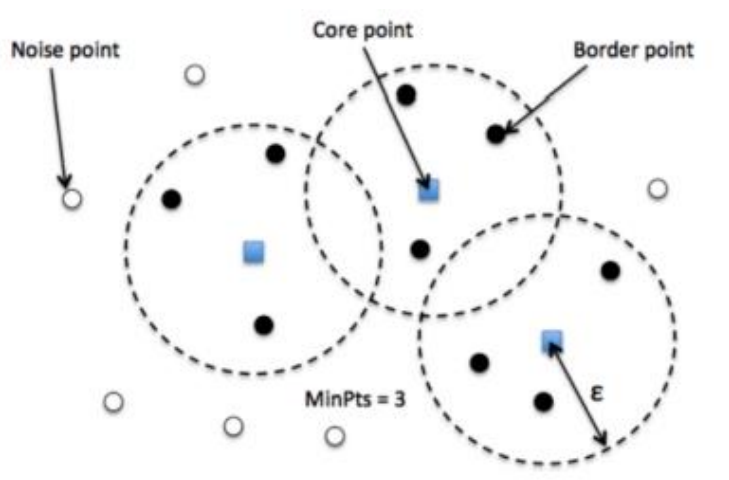
\includegraphics[width=0.8\linewidth]{dbscan.png}

\multend

\begin{KR}{Implementing DBSCAN}
\paragraph{Set parameters}
\begin{itemize}
    \item $\epsilon$: Maximum distance between points in the same neighborhood
    \item minPts: Minimum number of points required to form a dense region
\end{itemize}

\paragraph{Classify points}
For each unvisited point $P$:
\begin{itemize}
    \item Mark $P$ as visited
    \item Find all points within distance $\epsilon$ of $P$ (its neighborhood)
    \item If neighborhood has fewer than minPts, mark $P$ as noise (can be changed later)
    \item If neighborhood has at least minPts, start a new cluster with $P$ as a core point
\end{itemize}

\paragraph{Expand clusters}
For each core point $P$ in a cluster:
\begin{itemize}
    \item Find all points in the $\epsilon$-neighborhood of $P$
    \item For each point $Q$ in the neighborhood:
    \begin{itemize}
        \item If $Q$ is unvisited or marked as noise, add it to the cluster
        \item If $Q$ is a core point, recursively expand the cluster from $Q$
    \end{itemize}
\end{itemize}
\end{KR}

\mult{2}

\begin{concept}{Advantages of DBSCAN}

    Doesn't require specifying the number of clusters in advance

    Can find arbitrarily shaped clusters, not just spherical ones

     Robust to outliers (identifies them as noise points)

     Only needs two parameters ($\epsilon$ and minPts)

     Can handle clusters of different sizes and densities (to some extent)

\end{concept}

\begin{concept}{Limitations of DBSCAN}
\begin{itemize}
    \item Struggles with varying density clusters
    \item Sensitive to parameter choices
    \item Doesn't work well with high-dimensional data due to the ''curse of dimensionality''
    \item Not deterministic when points can be reached through multiple paths
    \item Computationally expensive for large datasets (though optimized implementations exist)
\end{itemize}
\end{concept}

\multend

\begin{example}{DBSCAN Application}
Consider identifying geographical regions in a city based on crime density:
\begin{itemize}
    \item Data: Latitude and longitude coordinates of crime incidents
    \item Parameters: $\epsilon = 0.5$ km, minPts = 10
    \item Results:
    \begin{itemize}
        \item Cluster 1: Downtown area with high crime density
        \item Cluster 2: Entertainment district with moderate crime
        \item Cluster 3: Shopping mall area with focused retail theft
        \item Noise points: Isolated incidents throughout the city
    \end{itemize}
    \item Advantages: Naturally identifies crime hotspots without predefined number of clusters
\end{itemize}
\end{example}

\subsection{Distance Metrics}

\begin{definition}{Common Distance Metrics}\\
The choice of distance metric affects clustering results:
\begin{itemize}
    \item \textbf{Euclidean Distance}: $d(p, q) = \sqrt{\sum_{i=1}^{N} (q_i - p_i)^2}$ (standard straight-line distance)
    \item \textbf{Manhattan Distance}: $d(p, q) = \sum_{i=1}^{N} |q_i - p_i|$ (sum of absolute differences)
    \item \textbf{Maximum Distance}: $d(p, q) = \max_i |q_i - p_i|$ (largest difference along any dimension)
    \item \textbf{Cosine Similarity}: $d_{cos}(p, q) = \frac{\sum_{i=1}^{N} p_i q_i}{\sqrt{\sum_{i=1}^{N} p_i^2} \sqrt{\sum_{i=1}^{N} q_i^2}}$ (angle between vectors)
\end{itemize}
\end{definition}

\begin{KR}{Choosing the Right Distance Metric}
\paragraph{Understand the data}
\begin{itemize}
    \item Consider the nature of features (categorical vs. numerical)
    \item Consider the relative importance of features
    \item Consider the scale of different features
\end{itemize}

\paragraph{Consider the application domain}
\begin{itemize}
    \item Euclidean: Good for continuous data in low dimensions
    \item Manhattan: Good when movement is restricted along axes (e.g., city blocks)
    \item Cosine: Good for text documents or high-dimensional data where magnitude is less important
    \item Correlation-based: Good when patterns matter more than absolute values
\end{itemize}

\paragraph{Preprocessing matters}
\begin{itemize}
    \item Standardize or normalize features before clustering
    \item Consider dimensionality reduction for high-dimensional data
    \item Handle categorical variables appropriately (one-hot encoding, etc.)
\end{itemize}
\end{KR}

\subsection{Other Clustering Algorithms}

\begin{concept}{Hierarchical Clustering}\\
Hierarchical clustering builds a tree of clusters (dendrogram):
\begin{itemize}
    \item \textbf{Agglomerative (bottom-up)}: Start with each point as its own cluster, then merge closest clusters
    \item \textbf{Divisive (top-down)}: Start with all points in one cluster, then recursively divide
    \item Doesn't require specifying the number of clusters in advance
    \item Can visualize cluster structure at different levels
    \item Linkage methods (single, complete, average, Ward) determine how cluster distances are measured
\end{itemize}
\end{concept}

\begin{KR}{Hierarchical Clustering Steps}
    Step 1: Form initial clusters consisting of a single object and compute the distance between each pair of clusters

Step 2: Merge the two clusters having minimum distance
Step 3: Calculate the distance between the new cluster and all other clusters
Step 4: Repeat step 2 and 3 until there is only one cluster remaining
A Dendrogram is a tree of nodes representing clusters, satisfying the following properties:
- Root represents the whole data set
- Leaf nodes represent clusters containing a single object
- Inner nodes represent the union of all objects contained in its corresponding subtrees

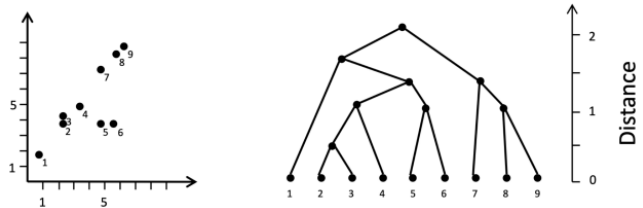
\includegraphics[width=\linewidth]{dendrogram.png}
\end{KR}

\begin{theorem}{Linkage in Hierarchical Clustering}\\
    Single Linkage: Shortest distance single link $(\min )$ between an element in one cluster and an element in the other, i.e., $d\left(C_i, C_j\right)=\min \left\{d\left(x_{i p}, x_{j q}\right)\right\}$.

Complete Linkage: Largest distance between an element in one cluster complete link (max) and an element in the other, i.e., $d\left(C_i, C_j\right)=\max \left\{d\left(x_{i p}, x_{j p}\right)\right\}$.

Average Linkage: Average distance between average elements in one cluster and elements in the other, i.e. $d\left(C_i, C_j\right)=\operatorname{avg}\left\{d\left(x_{i p}, x_{j p}\right)\right\}$.

\end{theorem}

\begin{example2}{Linkage Example}\\
    Clustering of the 1-dimensional data set $\{2, \mathbf{1 2}, \mathbf{1 6}, \mathbf{2 5}, \mathbf{2 9}, 45\}$

    1. Find lowest distance $\rightarrow(10,4,9,4,45)$ and build clusters
$
\{2,(12,16),(25,29), 45\}
$

2. Find lowest distance based on metrics and build clusters

- Centroid:
$
\{2,(12,16),(25,29), 45\} \rightarrow(12,13,18)
$, 
$
\{(\mathbf{2}, \mathbf{1 2}, \mathbf{1 6}),(25,29), 45\}
$

- Single:
$
\{2,(12,16),(25,29), 45\} \rightarrow(10,9,16)
$, 
$
\{2,(12,16,25,29), 45\}
$

- Complete:
$
\{2,(12,16),(25,29), 45\} \rightarrow(14,17,16)$, $
\{(2,12,16),(25,29), 45\}
$

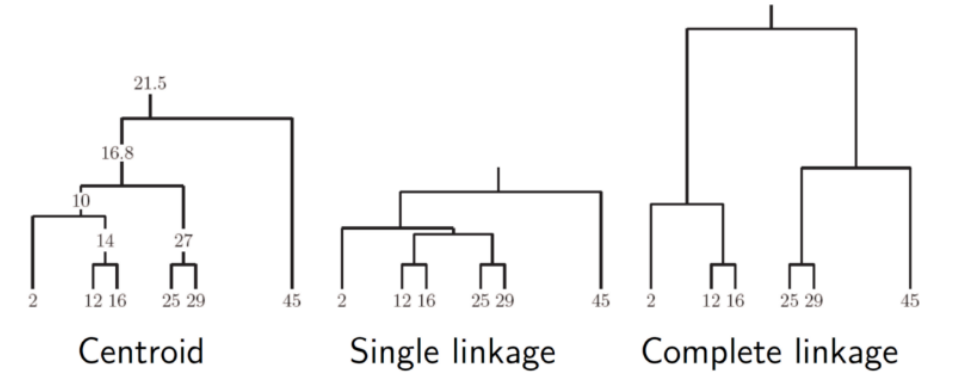
\includegraphics[width=0.7\linewidth]{linkage_example.png}
\end{example2}


\begin{concept}{Gaussian Mixture Models (GMM)}\\
GMMs are a probabilistic clustering approach:
\begin{itemize}
    \item Model the data as a mixture of several Gaussian distributions
    \item Each Gaussian component represents a cluster
    \item Provides soft cluster assignments (probabilities)
    \item Parameters estimated using Expectation-Maximization (EM) algorithm
    \item More flexible than K-means but more computationally intensive
\end{itemize}
\end{concept}

\begin{example2}{Comparison of Clustering Algorithms}\\
Consider clustering customer purchase behavior:
\begin{itemize}
    \item Features: Average purchase amount, purchase frequency, time since last purchase
    \item Dataset: 1000 customers
\end{itemize}
\tcblower
K-means:
\begin{itemize}
    \item Fast computation (convergence in 15 iterations)
    \item Creates spherical clusters of similar sizes
    \item Some customers don't fit well in any cluster
    \item Needs careful initialization
\end{itemize}

DBSCAN:
\begin{itemize}
    \item Identifies high-spending and frequent shopper clusters effectively
    \item Marks outliers (abnormal purchase patterns) as noise
    \item Doesn't force customers into clusters artificially
    \item More computationally expensive than K-means
\end{itemize}

Hierarchical Clustering:
\begin{itemize}
    \item Provides insight into relationships between clusters
    \item Shows that the high-spending cluster has two distinct sub-groups
    \item Most computationally expensive of the three
    \item Results sensitive to the linkage method chosen
\end{itemize}
\end{example2}

\begin{KR}{Implementing a Clustering Project}
\paragraph{Define the problem}
\begin{itemize}
    \item Clarify business objectives
    \item Understand what insights are needed
    \item Define what makes a ''good'' cluster in your context
\end{itemize}

\paragraph{Prepare the data}
\begin{itemize}
    \item Clean and preprocess data (handle missing values, outliers)
    \item Select relevant features
    \item Normalize or standardize features
    \item Consider dimensionality reduction if necessary
\end{itemize}

\paragraph{Choose and apply clustering algorithms}
\begin{itemize}
    \item Select appropriate algorithms based on data characteristics
    \item Try multiple algorithms and parameter settings
    \item Evaluate using internal validation metrics
\end{itemize}

\paragraph{Interpret and validate results}
\begin{itemize}
    \item Profile clusters to understand their characteristics
    \item Visualize clusters using dimensionality reduction (PCA, t-SNE)
    \item Validate with domain experts
    \item Test stability by rerunning with different samples
\end{itemize}

\paragraph{Implement findings}
\begin{itemize}
    \item Create actionable insights from clusters
    \item Develop a strategy to use clusters in business processes
    \item Set up a system to assign new data points to clusters
\end{itemize}
\end{KR}


\raggedcolumns
\pagebreak

\section{Association Rules and Pattern Mining}

\subsection{Association Rules}

\mult{2}

\begin{definition}{Association Rules Goal}\\
The goal of association rules is to find correlations between multiple items.
\end{definition}


\begin{definition}{Support Count and Support}
\begin{itemize}
    \item \textbf{support count} ($\sigma$): frequency of itemsets
    \item \textbf{support} ($s$): fraction of transactions that contain an itemset
    \item \textbf{confidence} ($c$): how often items in $Y$ appear in transactions that contain $X$
\end{itemize}

$$c = \frac{\sigma(X \cup Y)}{\sigma(X)}$$
\end{definition}



\begin{definition}{Frequent Itemset}\\
A frequent itemset is an itemset whose support is greater than or equal to a minimum support threshold.
\end{definition}

\begin{definition}{Association Rule}\\
An association rule is an implication expression of the form $X \rightarrow Y$ where $X$ and $Y$ are frequent itemsets.

Example: $\{milk, bread\} \rightarrow \{honey\}$
\end{definition}

\begin{definition}{Association Rule Mining Goal}\\
Given a set of transactions $T$, the goal of association rule mining is to find all rules having:
$$s \geq min\_s\_threshold, \quad c \geq min\_c\_threshold$$
\end{definition}


\begin{formula}{Lift}\\
Lift measures for how likely item $Y$ is purchased when item $X$ is purchased, while controlling for how popular item $Y$ is.

$$lift(x \rightarrow y) = \frac{support(x, y)}{support(x) \cdot support(y)}$$

\begin{itemize}
    \item $lift \approx 1$ implies no association
    \item $lift < 1$ implies negative association
    \item $lift > 1$ implies positive association
\end{itemize}
\end{formula}

\begin{example2}{One-Dimensional Example}\\
$buys(X, iPhone) \rightarrow buys(X, charging\_cable)$

$s = 18$, $c = 63$
\begin{itemize}
    \item 18\% of all transactions showed that an iPhone and a charging cable were bought together
    \item 63\% of customers that bought an iPhone also bought a charging cable
\end{itemize}
\end{example2}

\begin{example2}{Multi-Dimensional Example}\\
$age(X, [20,\ldots,29]) \land income(X, [40k,\ldots,49k]) \rightarrow buys(X, iPhone)$

$s = 2$, $c = 60$
\end{example2}




\multend

\begin{example2}{Association Rule Example}\\
    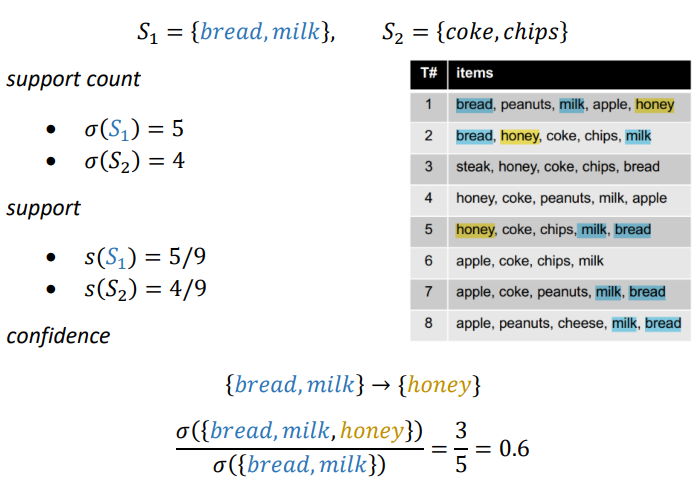
\includegraphics[width=0.8\linewidth]{association_rule_example.png}
\end{example2}


\raggedcolumns
\columnbreak

\subsection{Frequent Pattern Mining}

\begin{concept}{Exponential Growth Problem}\\
The possible number of frequent itemsets is huge. If an itemset is frequent, each of its subsets is frequent as well. For example, a frequent itemset of length 100 contains $\binom{100}{1} = 100$ frequent 1-itemsets, $\binom{100}{2} = 100$ frequent 2-itemsets. Meaning that there are $2^{100} - 1$ possible frequent itemsets.
\end{concept}

\begin{concept}{Optimization Strategies}
\begin{enumerate}
    \item Reduce the number of candidates $M$ by using pruning techniques
    \item Reduce the number of transactions $N$ by reducing the size of $N$ as the size of itemset increases
    \item Reduce the number of comparisons ($NM$) by using efficient data structures to store the candidates or transactions
\end{enumerate}
\end{concept}

\subsection{Apriori Algorithm}

\mult{2}

\begin{KR}{Apriori Algorithm to Generate Frequent Patterns}
Example with $\sigma_{min} = 2$

\paragraph{Step 1: Generate 1-itemset frequent pattern}
\begin{itemize}
    \item $C_1 =$ All 1-itemsets
    \item $L_1 =$ All 1-itemsets with $s \geq s_{min}$
\end{itemize}


\paragraph{Step 2: Generate 2-itemset frequent pattern}
\begin{itemize}
    \item $C_2 =$ All 2-itemsets ($L_1 \bowtie L_1$)
    \item $L_2 =$ All 2-itemsets $C_2$ with $s \geq s_{min}$
\end{itemize}


\paragraph{Step 3: Generate 3-itemset frequent pattern}
\begin{itemize}
    \item $C_3 =$ All 3-itemsets ($L_2 \bowtie L_2$)
    \item $L_3 =$ All 3-itemsets with $s \geq s_{min}$
\end{itemize}


\paragraph{Step 4: Generate 4-itemset frequent pattern}
\begin{itemize}
    \item $C_4 =$ All 4-itemsets ($L_3 \bowtie L_3$) $\rightarrow$ $\{coke, chips, ice, whiskey\}$ ($s = 1$)
    \item $L_4 = \{\}$
\end{itemize}

\paragraph{Steps 5 + 6: Generate association rules from frequent itemsets}
For every itemset in $L_n = (L_1, L_2, \ldots)$:
\begin{enumerate}
    \item Generate rules
    \item Check if $\frac{\sigma(I)}{\sigma(S)} = c \geq minc$ where $minc = 0.7 = 70\%$
\end{enumerate}
\end{KR}

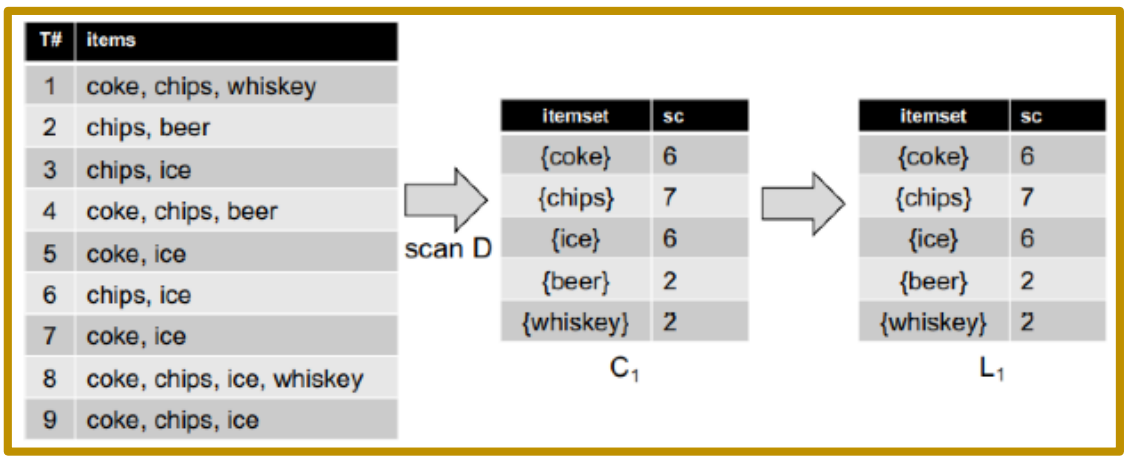
\includegraphics[width=\linewidth]{apriori1.png}

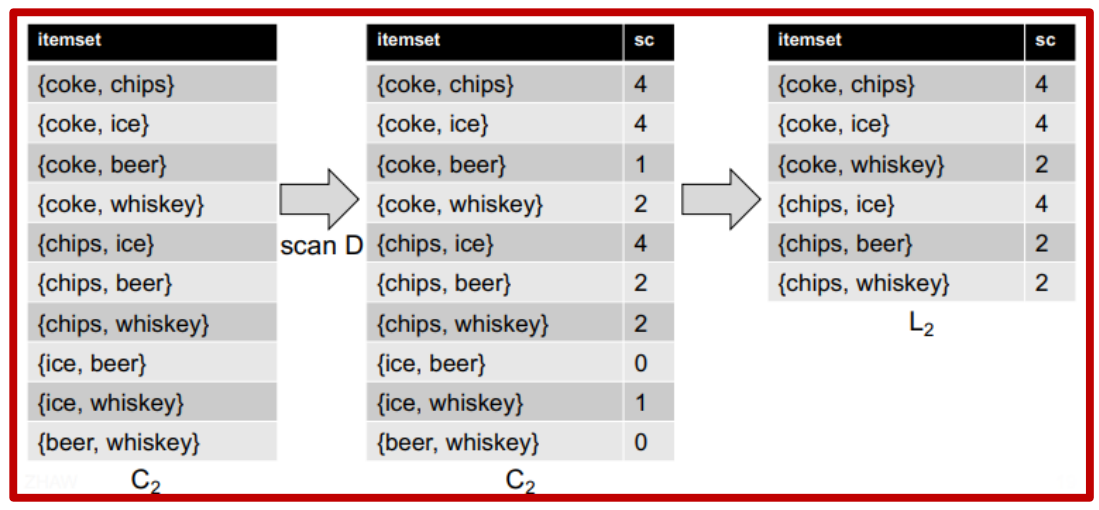
\includegraphics[width=\linewidth]{apriori2.png}

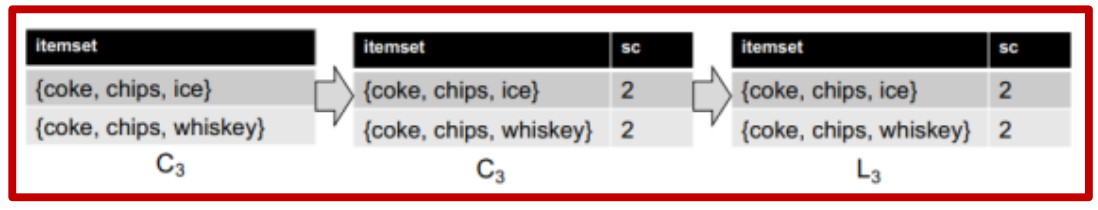
\includegraphics[width=\linewidth]{apriori3.png}

\multend

\begin{example2}{Rule Generation Example}
Example: $I = \{coke, chips, whiskey\}$

\textbf{Rule1}: $S = \{coke, chips\} \rightarrow \{whiskey\} \rightarrow$
$c = \frac{\sigma(I)}{\sigma(S)} = \frac{2}{4} \rightarrow 0.5 = 50\% \rightarrow \text{rejected}$

\textbf{Rule2}: $S = \{coke, whiskey\} \rightarrow \{chips\} \rightarrow$
$c = \frac{\sigma(I)}{\sigma(S)} = \frac{2}{2} \rightarrow 1 = 100\% \rightarrow \text{accepted}$
\end{example2}

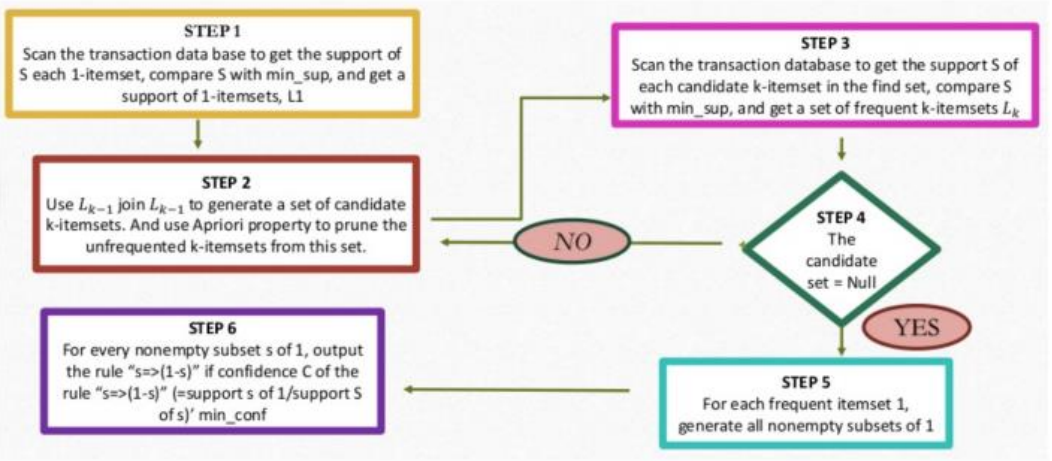
\includegraphics[width=0.8\linewidth]{apriori_flow_chart.png}

\subsection{FP-Tree Algorithm}

\begin{KR}{FP-Tree Construction}\\
    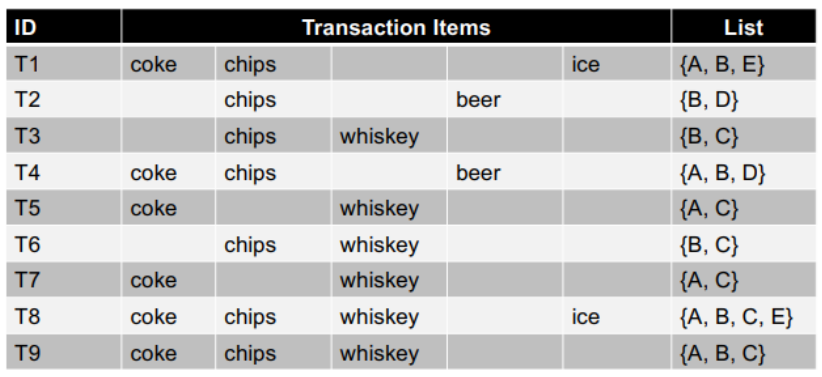
\includegraphics[width=0.8\linewidth]{fptree1.png}

\paragraph{Step 1: Calculate min support count $min\sigma$}
$min\_s = 22\% \rightarrow min\sigma = 0.22 \cdot 9 = 1.98 \rightarrow 2$

\paragraph{Step 2: Find frequency of occurrence $\sigma$ of each item}
\begin{itemize}
    \item A: Coke $\sigma = 6$
    \item B: Chips $\sigma = 7$
    \item C: Whiskey $\sigma = 6$
    \item D: Beer $\sigma = 2$
    \item E: Ice $\sigma = 2$
\end{itemize}
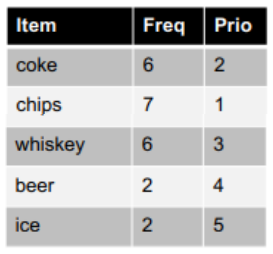
\includegraphics[width=0.2\linewidth]{fptree2.png}

\paragraph{Step 3: Order the items according to priority}
$\{A, B, E\} \rightarrow \{B, A, E\}$\\
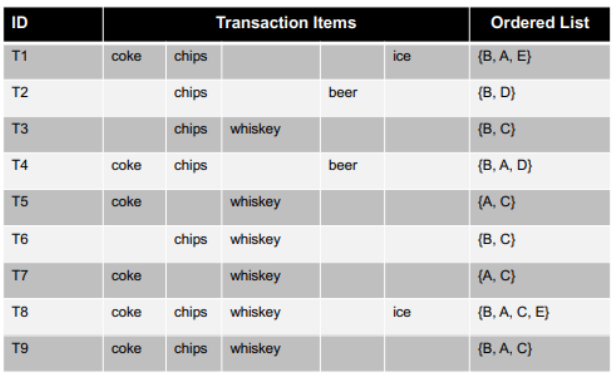
\includegraphics[width=0.7\linewidth]{fptree3.png}

\end{KR}

\begin{KR}{FP-Tree Construction Continued}

\paragraph{Step 4: Build the FP-Tree}
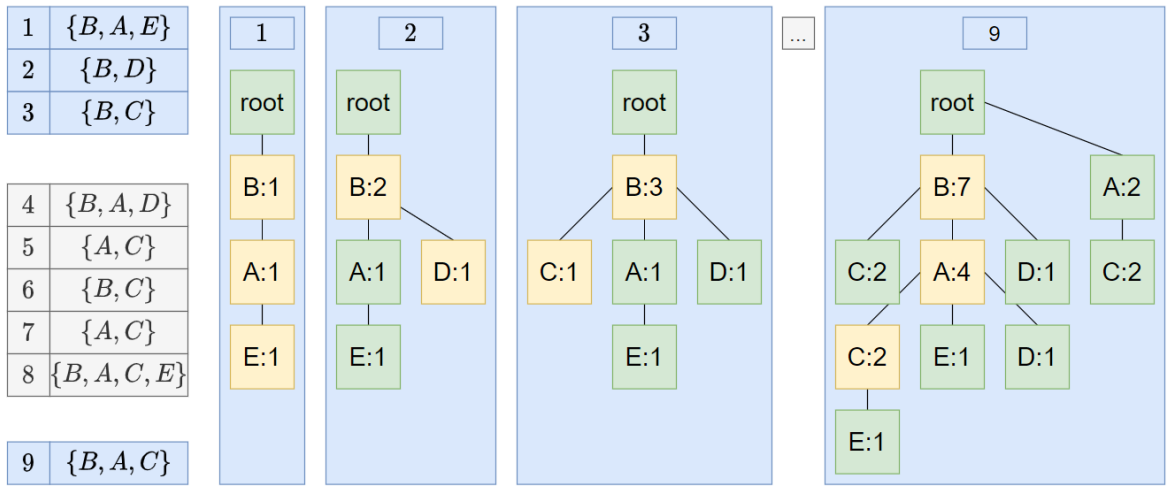
\includegraphics[width=\linewidth]{fptree4.png}

\paragraph{Step 5: Find conditional pattern base and conditional FP-Tree for each item}
\begin{itemize}
    \item $E: \{B, A: 2\}$
    \item $D: \{B: 2\}$
    \item $C: \{B: 4, A: 2\}, \{A: 2\}$
    \item $A: \{B: 4\}$
\end{itemize}
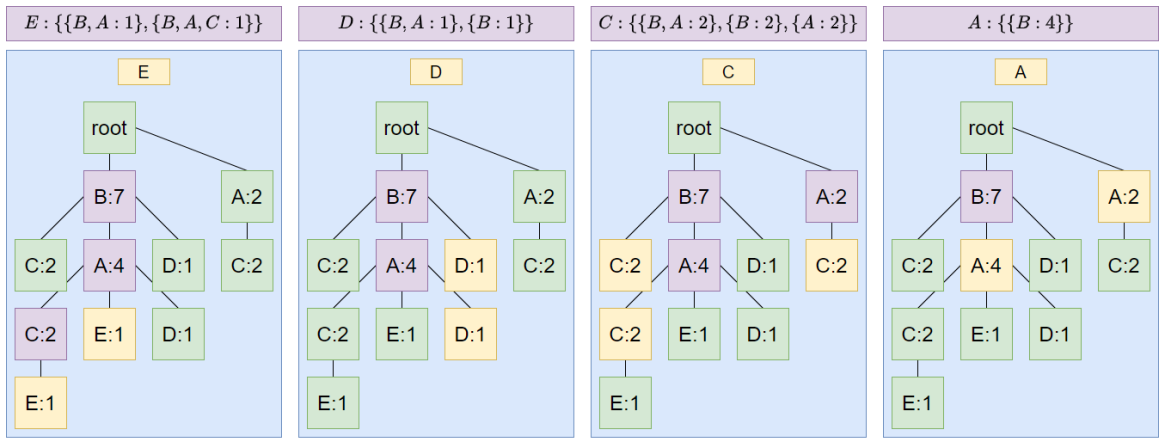
\includegraphics[width=\linewidth]{fptree5.png}
\end{KR}

\raggedcolumns
\pagebreak


\section{Recommender Systems}

\begin{definition}{Good Recommender System}
\begin{itemize}
    \item Recommends personalized and valuable items within the current context
    \item Recommends items from all different and possible areas of interest
    \item Does not recommend items which are already known
    \item Extends the areas of interest (serendipity effect)
\end{itemize}
\end{definition}

\subsection{Collaborative Filtering}

\begin{concept}{Collaborative Filtering}\\
Analysis of behaviour patterns of user groups. Recommends items to a user based on comparison of their behaviour against users with a ''similar'' behaviour.
\end{concept}

\begin{formula}{Cosine Similarity}
$$similarity = \cos(\theta) = \frac{A \cdot B}{||A|| \cdot ||B||} = \frac{\sum_{i=1}^{n} A_i B_i}{\sqrt{\sum_{i=1}^{n} A_i^2} \cdot \sqrt{\sum_{i=1}^{n} B_i^2}}$$
\end{formula}

\begin{concept}{Challenges in Recommender Systems}
\begin{itemize}
    \item Many items to recommend, but only a few can be recommended
    \item Mostly sparse data per user
    \item Interest measure can be very diverse (Explicit: ratings, Implicit: clicks)
    \item No data for new users
\end{itemize}
\end{concept}

\subsection{Types of Filtering}

\begin{definition}{Content-Based Collaborative Filtering}\\
Recommendations are based on the content or the attributes of the objects instead of the user behaviour and ratings. There are explicit attributes and the content of an object.
\end{definition}

\begin{definition}{Context-Aware Filtering}\\
Filtering based on a dynamic collection of factors that describe the status of a user (time, location, social factor).
\end{definition}

\subsection{User-Based Collaborative Filtering}

\begin{concept}{User-Based Collaborative Filtering}\\
Calculates the similarity between the users based on their rating behaviour.
\end{concept}

\begin{example2}{User Similarity Example}\\
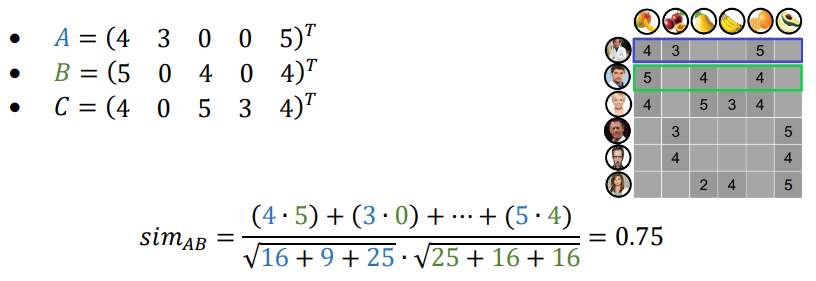
\includegraphics[width=0.8\linewidth]{collaborative_filtering1.png}

Recommend items with a high rating from these similar users:

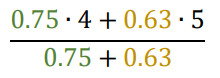
\includegraphics[width=0.3\linewidth]{dkfjdklhgdh.png}
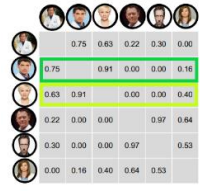
\includegraphics[width=0.3\linewidth]{collaborative_filtering2.png}
\end{example2}


\subsection{Item-Based Collaborative Filtering}

\begin{concept}{Item-Based Collaborative Filtering}\\
Calculates the similarity between the items based on their rating.
\end{concept}

\begin{example2}{Item Similarity Example}\\
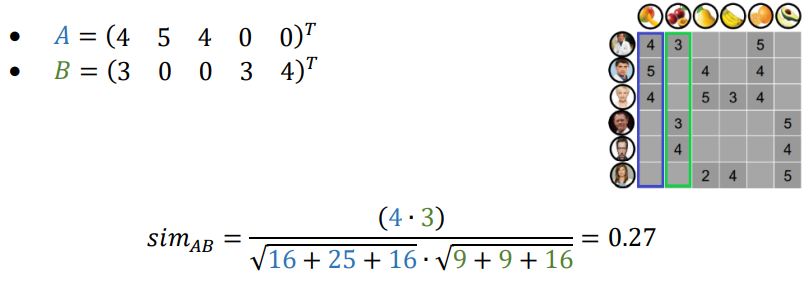
\includegraphics[width=0.8\linewidth]{itembased_filtering.png}

Recommends the most similar items with the highest ranking.
\end{example2}
